\subsubsection{JupyterLab Servers}

\newline
OpenSciencLabs are JupyterHubs running on Kubernetes clusters in the cloud. When a user starts a server, they are assigned a compute pod running JupyterLab on the cluster, their perisitent storage volume is mounted, and a script runs to help prepare their environment.

Depending on the lab, users typically have access to multiple server profiles, designed to suit the needs of a given workflow. Cloud computing is expensive, so it important to select a server that is powerful enough while avoiding an oversized, wasteful configuration.

\begin{framed}
\textbf{OpenSARLab offers 2 default server profiles}\\
\textbf{m6a.large Server:}

\begin{itemize}
\item RAM Guarantee: 5G
\item RAM limit: 8G
\item CPU limit: 2
\end{itemize}

\textbf{m6a.xlarge Server:}

\begin{itemize}
\item RAM Guarantee: 10G
\item RAM limit: 16G
\item CPU limit: 4
\end{itemize}
\end{framed}

\begin{itemize}
\item What~happens~when~a~server~is~started?
\item How~to~Start~and~Stop~a~Server
\end{itemize}


\bigskip
\centerline{\rule{13cm}{0.4pt}}
\bigskip

\paragraph{What happens when a server is started?}\label{What-happens-when-a-server-is-started}

When a user starts a server, they are assigned a compute pod on a node in the lab's Kubernetes cluster. A Docker container runs JupyterLab on the pod and the user's volume is mounted. Next, a shell script runs making some final adjustments to the environment and updating any lab-provided Jupyter Notebook repositories with the notebook repository synching tool, \texttt{nbgitpuller}. Finally, the user accesses their server and Jupyter Lab instance via a web browser.

\begin{framed}
\textbf{Reasons you may wish to restart a running lab server}\\
\begin{itemize}
\item Your workflows require additional resources, so you shut down the current server and select a more robust server profile.
\item You accidentally delete or change a notebook and wish to retrieve a fresh copy.\begin{itemize}
\item You can also run \texttt{nbgitpuller} from the terminal if you wish, but restarting the server is any easy way to pull in updates.
\end{itemize}
\end{itemize}
\end{framed}


\bigskip
\centerline{\rule{13cm}{0.4pt}}
\bigskip

\paragraph{How to Start and Stop a Server}\label{How-to-Start-and-Stop-a-Server}

\begin{framed}
\textbf{Please shut down you server after use}\\
Cloud computing is expensive. Keeping a dormant server running impacts the budget, reducing available funding for a lab and its users. Please act as a steward for you labs' resources by shutting down your servers when not in use.
\end{framed}

\subparagraph{Starting a Server}

\begin{enumerate}
\item Sign into  \href{https://opensciencelab.asf.alaska.edu/}{OpenScienceLab} and click the ``Go to lab'' button on the card of the lab you wish to start.
\end{enumerate}

\begin{figure}[!htbp]
\centering
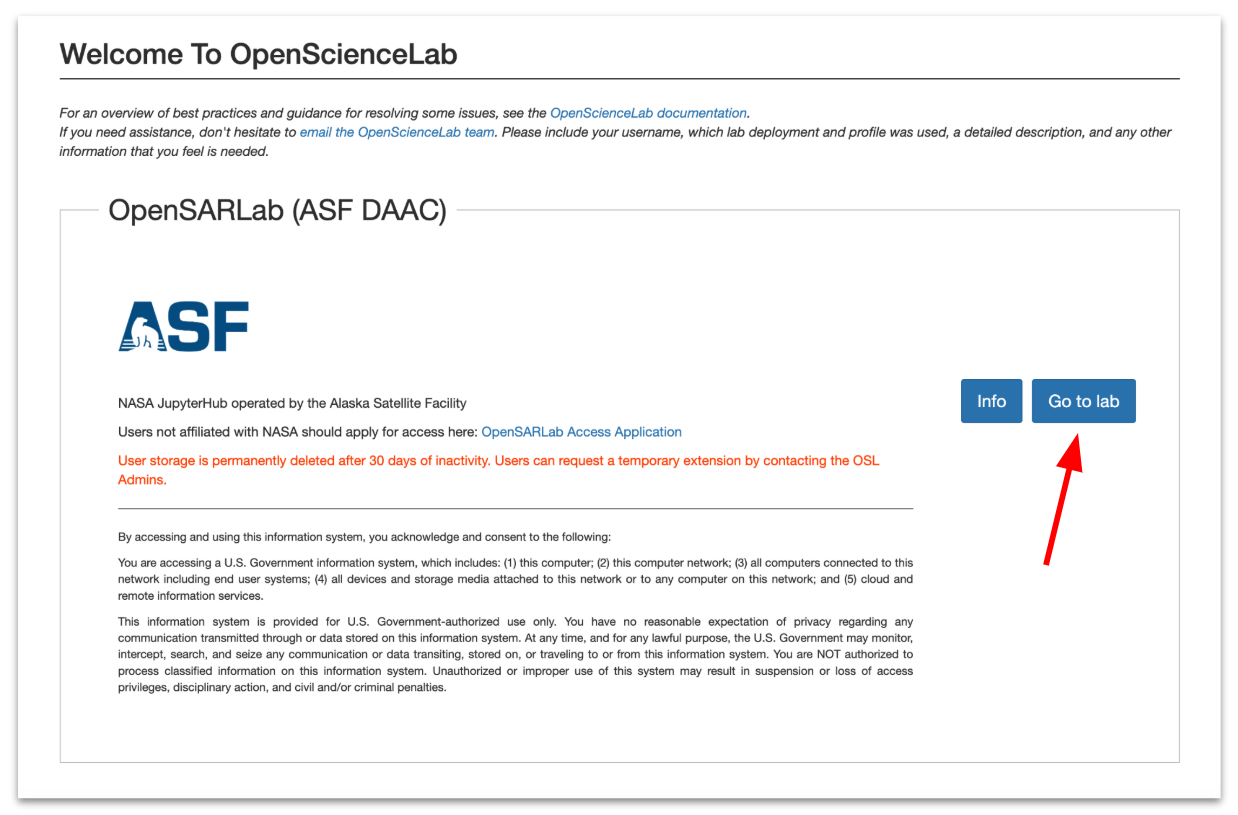
\includegraphics[width=0.7\linewidth]{files/opensciencelab_goto_-2d6003078519e1928c1d6adc33f7a29f.png}
\caption*{The OpenScienceLab Portal provides access to users' labs. In this example, there is only one lab available, but users will see lab cards for any labs to which they have access.}
\end{figure}

\begin{enumerate}[resume]
\item Click the \texttt{Start My Server} button.
\end{enumerate}

\begin{figure}[!htbp]
\centering
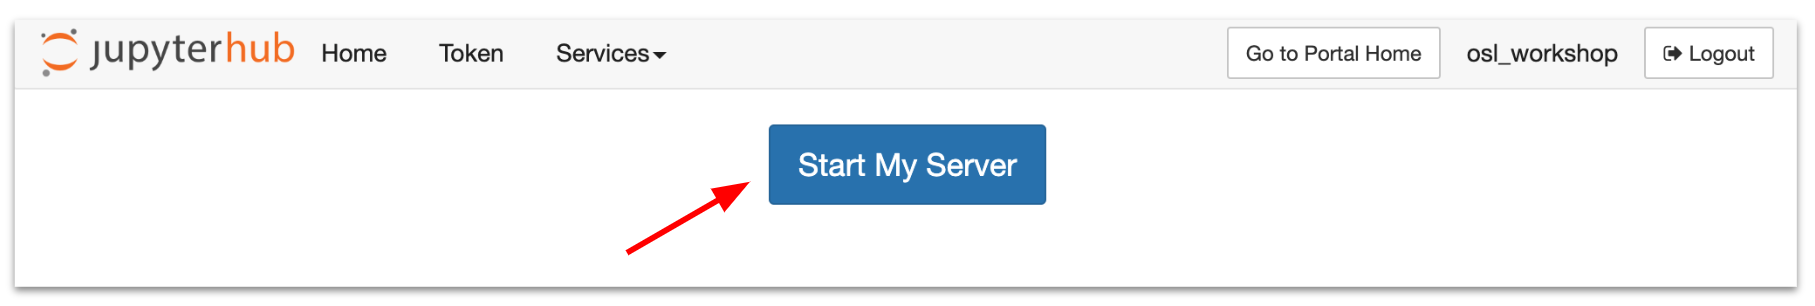
\includegraphics[width=0.7\linewidth]{files/start_server-f7c4d33c0700583fa6071e15002d6364.png}
\end{figure}

\begin{enumerate}[resume]
\item On the Server Options page, select the radio button of the server profile you wish to use and click the \texttt{Start} button.
\end{enumerate}

\begin{figure}[!htbp]
\centering
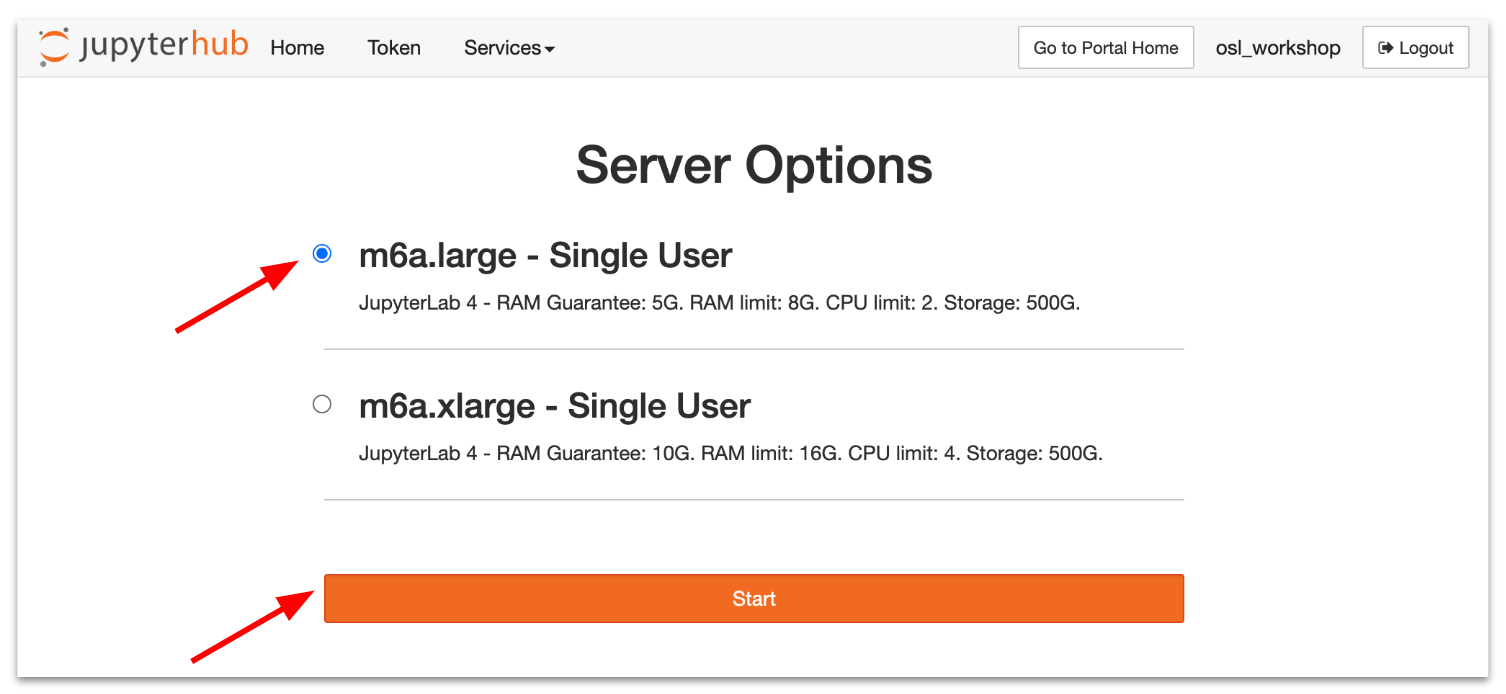
\includegraphics[width=0.7\linewidth]{files/server_profile_selec-04f0a0fc0dc0d4a8fa77778ddb497242.png}
\end{figure}

\begin{enumerate}[resume]
\item A status screen will load while your server starts.
\end{enumerate}

\begin{figure}[!htbp]
\centering
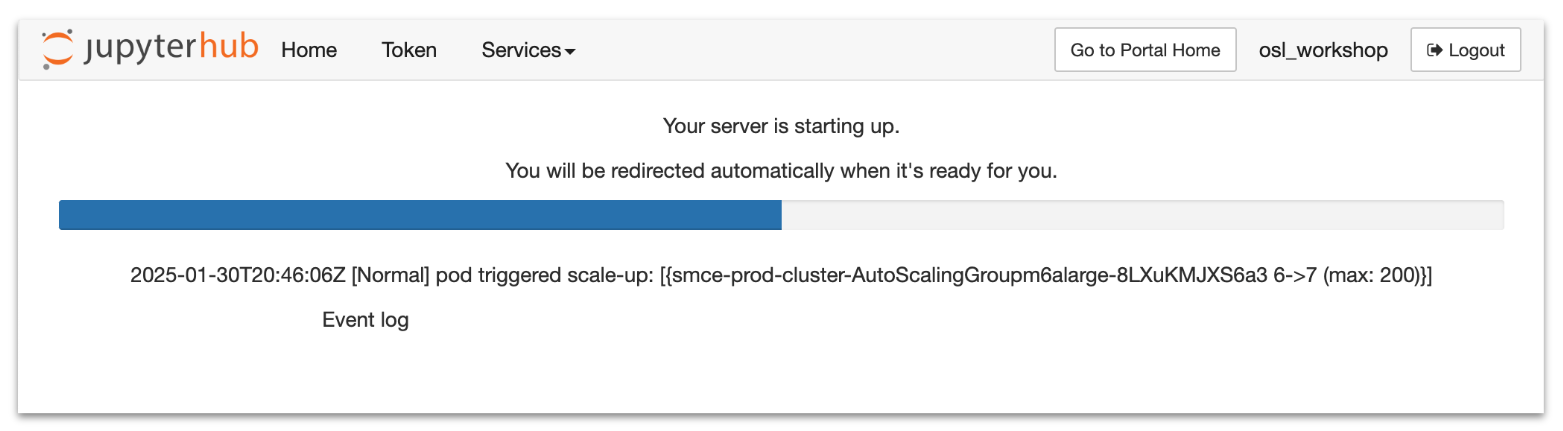
\includegraphics[width=0.7\linewidth]{files/server_status-bb8534988e98d7d4886c1eb6e2a8a7b1.png}
\end{figure}

\begin{enumerate}[resume]
\item You can click on ``Event Log'' to display the system logs as your server starts.
\end{enumerate}

\begin{figure}[!htbp]
\centering
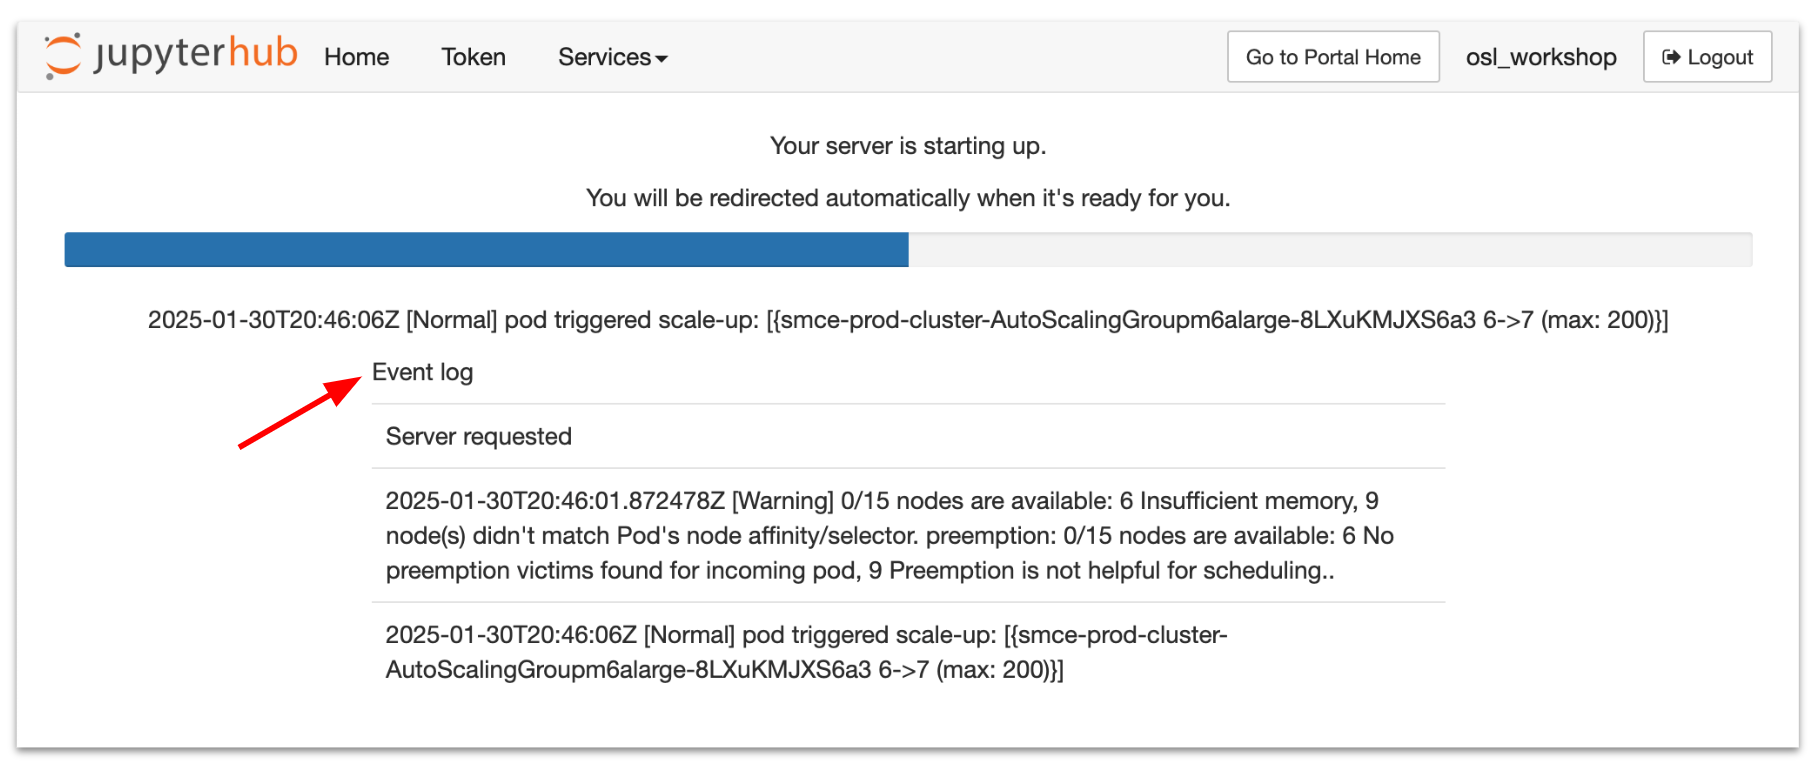
\includegraphics[width=0.7\linewidth]{files/event_log-a9d01375ba0ea46bdf88451ef1e3ecd3.png}
\end{figure}

\begin{enumerate}[resume]
\item It may take several minutes for a server to start. When it has started, you will have access to a JupyterLab desktop.
\end{enumerate}

\begin{figure}[!htbp]
\centering
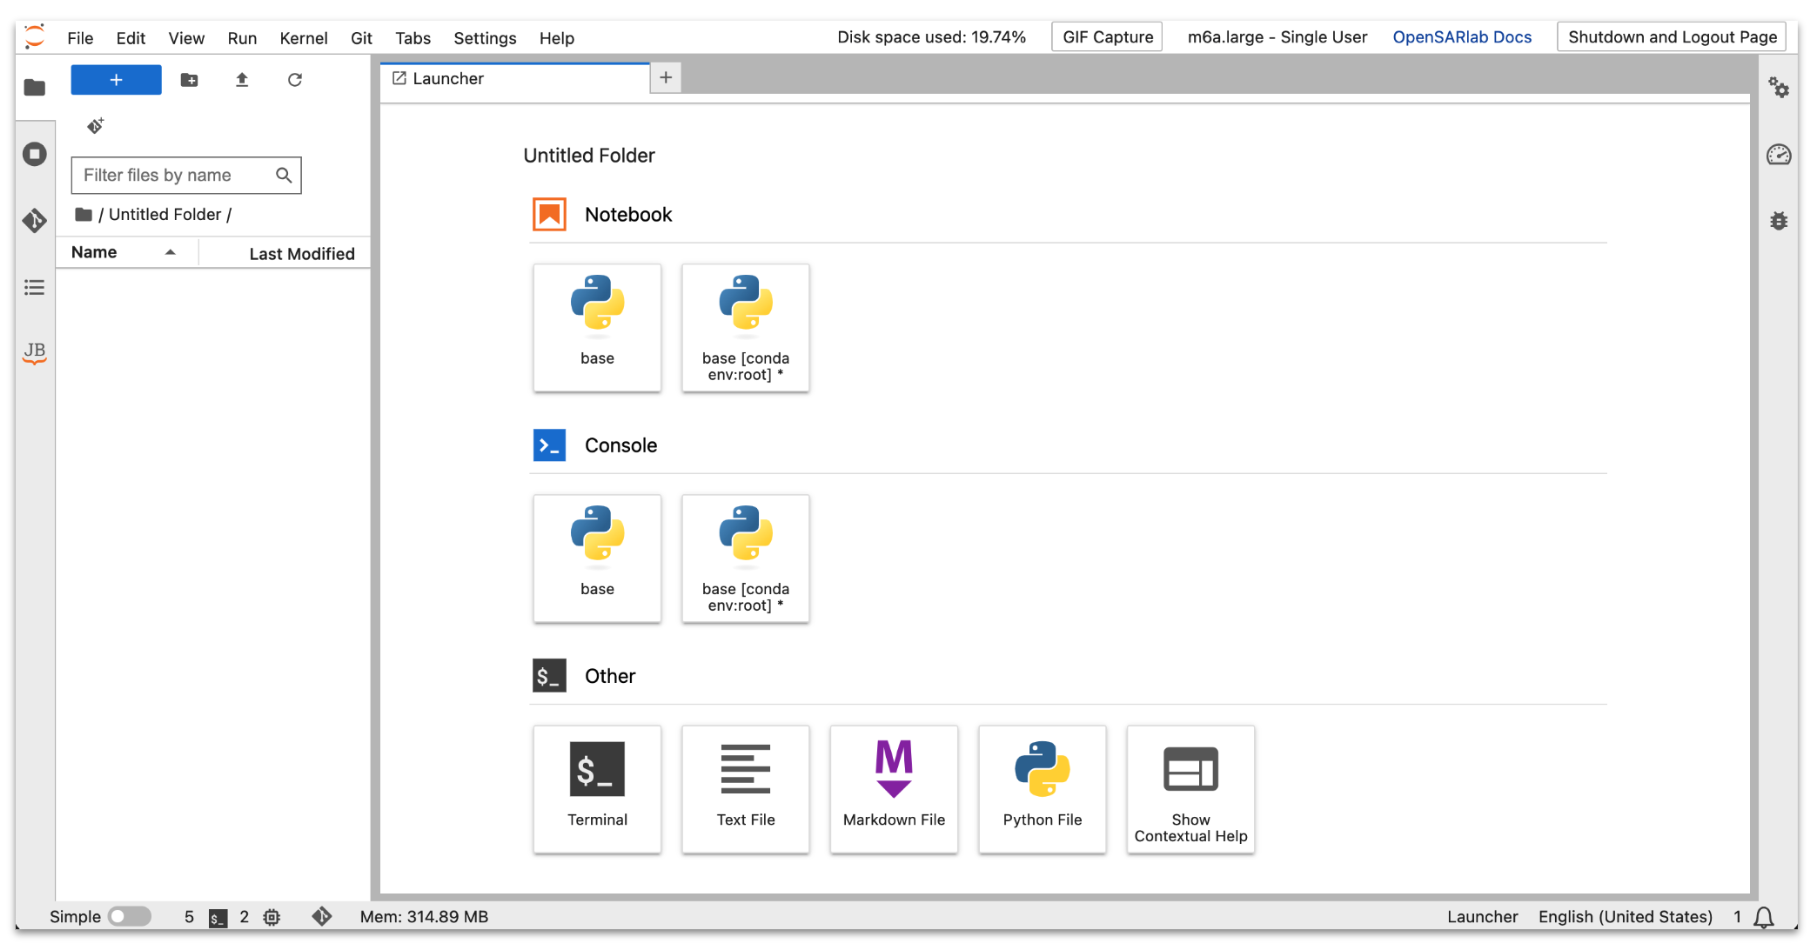
\includegraphics[width=0.7\linewidth]{files/jupyter_lab-fdc94447b7e46a4e672337bf84e8cf49.png}
\caption*{The JupyterLab desktop loads when your server has started. Depending on the specific lab, you may have access to varying notebook kernels and JupyterLab extensions.}
\end{figure}

\subparagraph{Stopping a Server}

\begin{enumerate}
\item Select \texttt{Hub Control Panel} from the \texttt{File} menu
\end{enumerate}

\begin{figure}[!htbp]
\centering
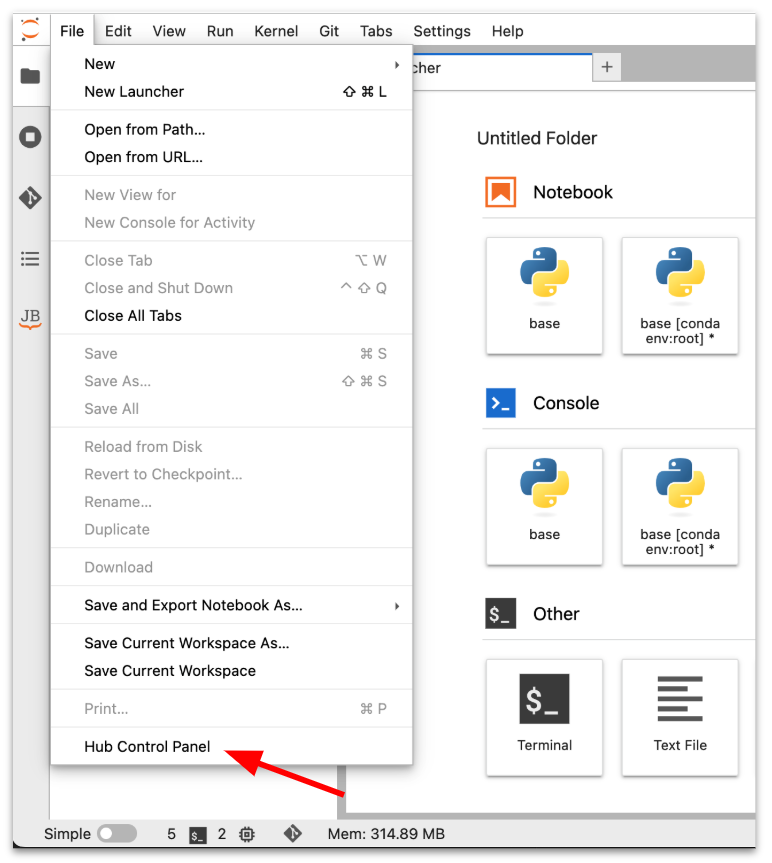
\includegraphics[width=0.7\linewidth]{files/jupyterhub_control_p-8d395ee205601c03418bf1a9e775c2d4.png}
\end{figure}

or

Click the \texttt{Shutdown and Logout Page} button at the top right of the JupyterLab desktop

\begin{figure}[!htbp]
\centering
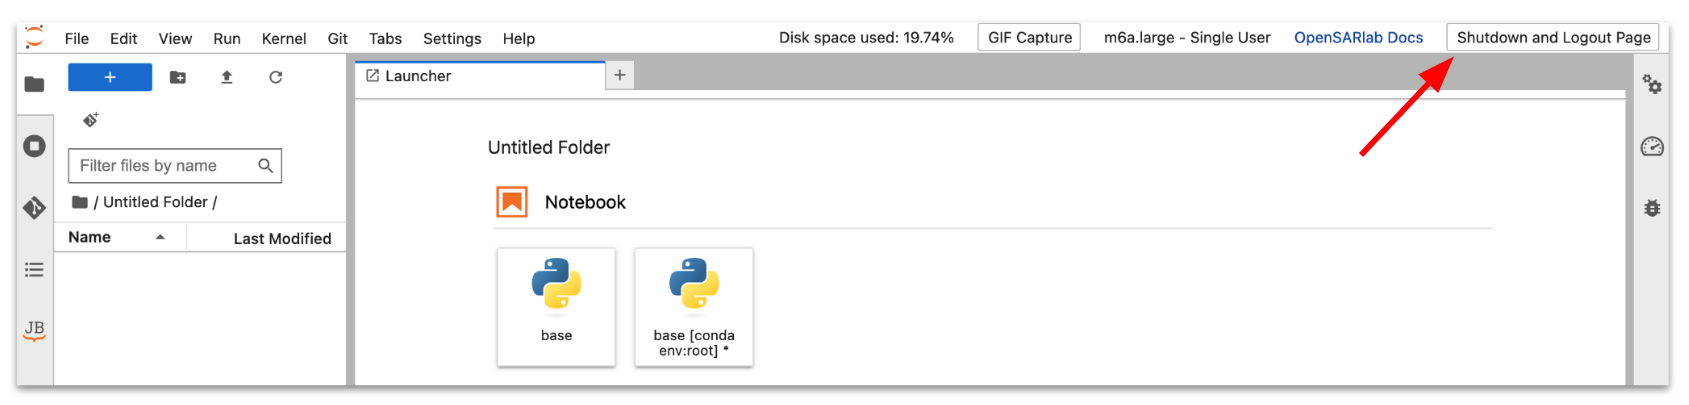
\includegraphics[width=0.7\linewidth]{files/shutdown_logout_butt-ebf28f7358ab734375ae40c2ef0d02e8.png}
\end{figure}

\begin{enumerate}[resume]
\item Click the \texttt{Stop My Server} Button
\end{enumerate}

\begin{figure}[!htbp]
\centering
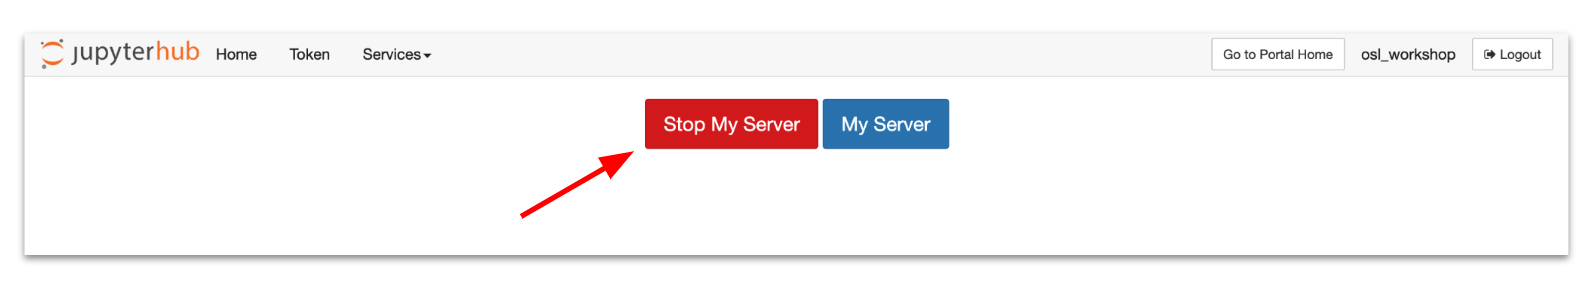
\includegraphics[width=0.7\linewidth]{files/stop_my_server-e8375d436e19a65eefdcf23fe9079287.png}
\end{figure}